\section{Blades Data}

\subsection{Blades Airfoils}

\begin{figure}[h!]
  \centering
  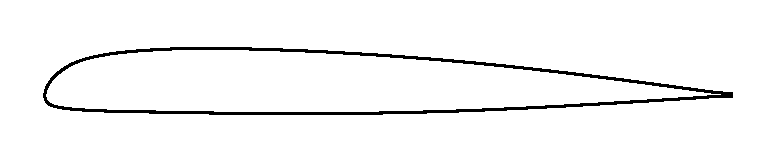
\includegraphics[width=127mm]{eps/airfoil_SC1094R8.eps}
  \caption{SC1094 R8}
\end{figure}

\begin{figure}[h!]
  \centering
  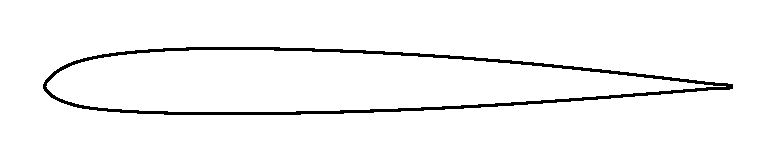
\includegraphics[width=127mm]{eps/airfoil_SC1095.eps}
  \caption{SC1095}
\end{figure}

\subsubsection{Ordinates}

\paragraph{SC1094 R8} ~

\csvreader[
  no head,
  longtable=cccc,
  table head=
    \toprule
    \multicolumn{2}{c}{\bfseries Upper surface} & \multicolumn{2}{c}{\bfseries Lower surface} \\
    x/c & y/c & x/c & y/c \\ \midrule
    \endfirsthead
    \multicolumn{2}{c}{\bfseries Upper surface} & \multicolumn{2}{c}{\bfseries Lower surface} \\
    x/c & y/c & x/c & y/c \\ \midrule
    \endhead,
  before first line={},
  late after line=\\,
  late after last line=\\ \bottomrule \caption{SC1094 R8 \cite{NASA-TP-2003-212265}},
  before reading={},
  after reading={}
]
{csv/airfoil_SC1094R8.csv}
{1=\colxu,2=\colyu,3=\colxl,4=\colyl}
{\colxu & \colyu & \colxl & \colyl}

\paragraph{SC1095} ~

\csvreader[
  no head,
  longtable=cccc,
  table head=
    \toprule
    \multicolumn{2}{c}{\bfseries Upper surface} & \multicolumn{2}{c}{\bfseries Lower surface} \\
    x/c & y/c & x/c & y/c \\ \midrule
    \endfirsthead
    \multicolumn{2}{c}{\bfseries Upper surface} & \multicolumn{2}{c}{\bfseries Lower surface} \\
    x/c & y/c & x/c & y/c \\ \midrule
    \endhead,
  before first line={},
  late after line=\\,
  late after last line=\\ \bottomrule \caption{SC1095 \cite{NASA-TP-2003-212265}},
  before reading={},
  after reading={}
]
{csv/airfoil_SC1095.csv}
{1=\colxu,2=\colyu,3=\colxl,4=\colyl}
{\colxu & \colyu & \colxl & \colyl}
